\documentclass{standalone}
\usepackage{tikz}
\usetikzlibrary{patterns, positioning}


\begin{document}
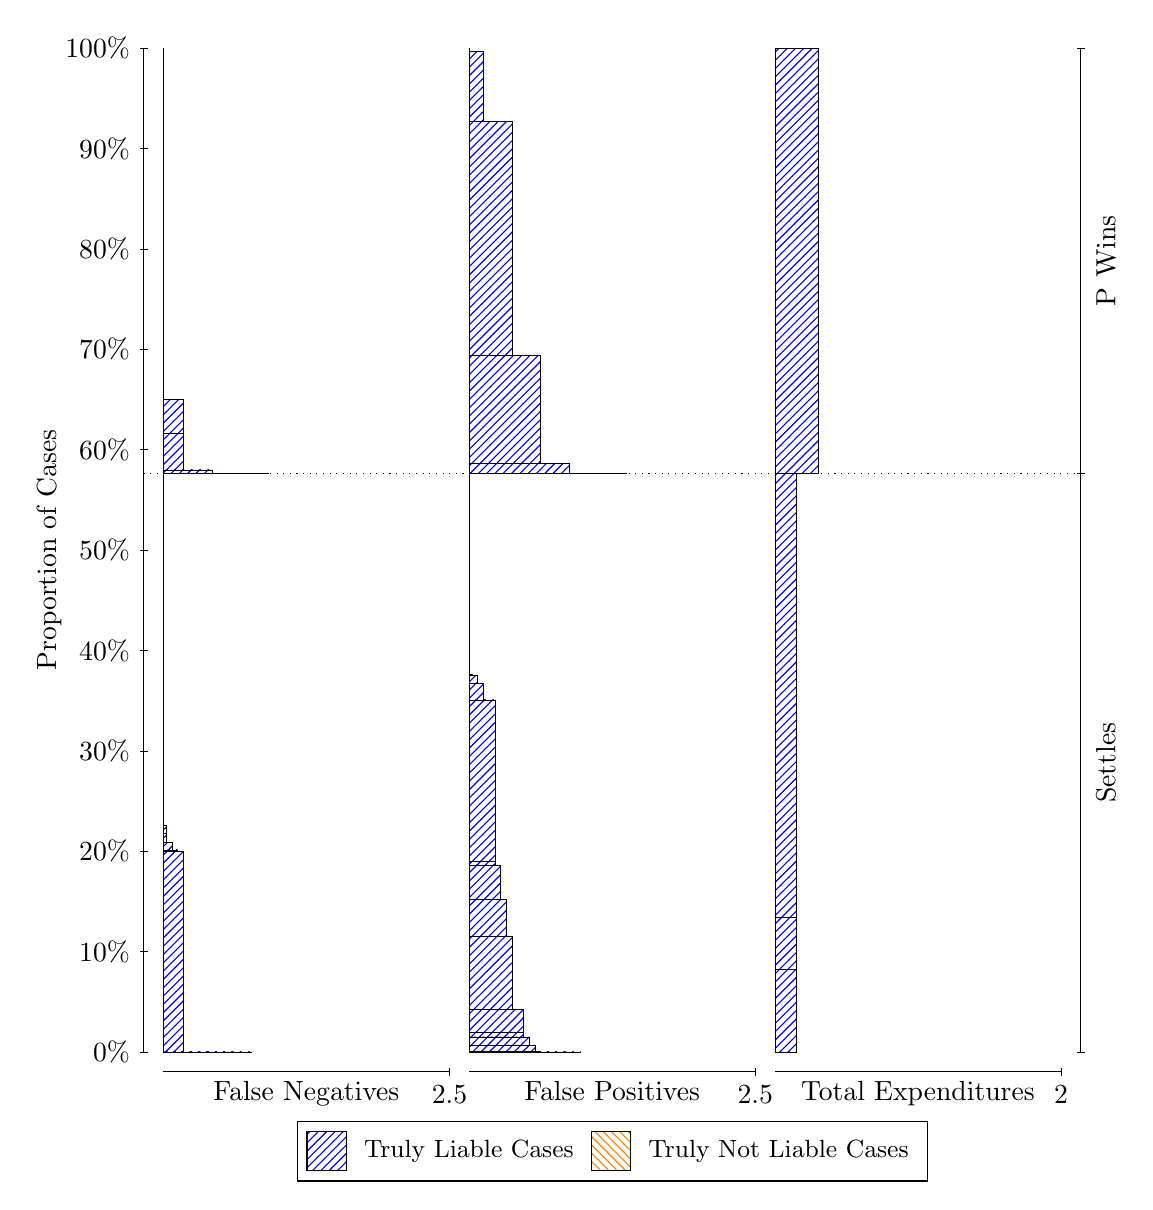
\begin{tikzpicture}
\draw[black, very thin] (1.5,1.75) -- (1.5,14.5);
\node[rotate=90, text=black, anchor=center] at (0.3, 8.125) {Proportion of Cases};
\draw[black, very thin] (1.45,1.75) -- (1.55,1.75);
\node[text=black, anchor=east] at (1.45, 1.75) {0\%};
\draw[black, very thin] (1.45,3.025) -- (1.55,3.025);
\node[text=black, anchor=east] at (1.45, 3.025) {10\%};
\draw[black, very thin] (1.45,4.3) -- (1.55,4.3);
\node[text=black, anchor=east] at (1.45, 4.3) {20\%};
\draw[black, very thin] (1.45,5.575) -- (1.55,5.575);
\node[text=black, anchor=east] at (1.45, 5.575) {30\%};
\draw[black, very thin] (1.45,6.85) -- (1.55,6.85);
\node[text=black, anchor=east] at (1.45, 6.85) {40\%};
\draw[black, very thin] (1.45,8.125) -- (1.55,8.125);
\node[text=black, anchor=east] at (1.45, 8.125) {50\%};
\draw[black, very thin] (1.45,9.4) -- (1.55,9.4);
\node[text=black, anchor=east] at (1.45, 9.4) {60\%};
\draw[black, very thin] (1.45,10.675) -- (1.55,10.675);
\node[text=black, anchor=east] at (1.45, 10.675) {70\%};
\draw[black, very thin] (1.45,11.95) -- (1.55,11.95);
\node[text=black, anchor=east] at (1.45, 11.95) {80\%};
\draw[black, very thin] (1.45,13.225) -- (1.55,13.225);
\node[text=black, anchor=east] at (1.45, 13.225) {90\%};
\draw[black, very thin] (1.45,14.5) -- (1.55,14.5);
\node[text=black, anchor=east] at (1.45, 14.5) {100\%};

\draw[black, very thin] (13.4,1.75) -- (13.4,14.5);
\draw[black, very thin] (13.35,1.75) -- (13.45,1.75);
\node[anchor=west] at (13.35, 1.75) {};
\draw[black, very thin] (13.35,9.0968) -- (13.45,9.0968);
\node[anchor=west] at (13.35, 9.0968) {};
\draw[black, very thin] (13.35,14.5) -- (13.45,14.5);
\node[anchor=west] at (13.35, 14.5) {};

\draw[black, very thin, pattern color=blue, pattern=north east lines] (1.75,1.75) rectangle (2.8763,1.75);
\draw[black, very thin, pattern color=blue, pattern=north east lines] (1.75,1.75) rectangle (2.731,1.75);
\draw[black, very thin, pattern color=blue, pattern=north east lines] (1.75,1.75) rectangle (2.5857,1.75);
\draw[black, very thin, pattern color=blue, pattern=north east lines] (1.75,1.75) rectangle (2.513,1.75);
\draw[black, very thin, pattern color=blue, pattern=north east lines] (1.75,1.75) rectangle (2.4403,1.75);
\draw[black, very thin, pattern color=blue, pattern=north east lines] (1.75,1.75) rectangle (2.3677,1.75);
\draw[black, very thin, pattern color=blue, pattern=north east lines] (1.75,1.75) rectangle (2.295,1.75);
\draw[black, very thin, pattern color=blue, pattern=north east lines] (1.75,1.75) rectangle (2.2223,1.7502);
\draw[black, very thin, pattern color=blue, pattern=north east lines] (1.75,1.7502) rectangle (2.1497,1.7507);
\draw[black, very thin, pattern color=blue, pattern=north east lines] (1.75,1.7507) rectangle (2.1497,1.7518);
\draw[black, very thin, pattern color=blue, pattern=north east lines] (1.75,1.7518) rectangle (2.077,1.7518);
\draw[black, very thin, pattern color=blue, pattern=north east lines] (1.75,1.7518) rectangle (2.0043,1.7522);
\draw[black, very thin, pattern color=blue, pattern=north east lines] (1.75,1.7522) rectangle (2.0043,4.2969);
\draw[black, very thin, pattern color=blue, pattern=north east lines] (1.75,4.2969) rectangle (1.9317,4.316);
\draw[black, very thin, pattern color=blue, pattern=north east lines] (1.75,4.316) rectangle (1.859,4.413);
\draw[black, very thin, pattern color=blue, pattern=north east lines] (1.75,4.413) rectangle (1.7863,4.5276);
\draw[black, very thin, pattern color=blue, pattern=north east lines] (1.75,4.5276) rectangle (1.7863,4.6249);
\draw[black, very thin, pattern color=orange, pattern=north west lines] (1.75,4.6249) rectangle (1.75,4.6249);
\draw[black, very thin, pattern color=blue, pattern=north east lines] (1.75,4.6249) rectangle (1.75,9.0968);
\draw[black, very thin, pattern color=blue, pattern=north east lines] (1.75,9.0968) rectangle (3.0943,9.0968);
\draw[black, very thin, pattern color=blue, pattern=north east lines] (1.75,9.0968) rectangle (2.731,9.097);
\draw[black, very thin, pattern color=blue, pattern=north east lines] (1.75,9.097) rectangle (2.3677,9.1423);
\draw[black, very thin, pattern color=blue, pattern=north east lines] (1.75,9.1423) rectangle (2.0043,9.6092);
\draw[black, very thin, pattern color=blue, pattern=north east lines] (1.75,9.6092) rectangle (2.0043,10.033);
\draw[black, very thin, pattern color=orange, pattern=north west lines] (1.75,10.033) rectangle (1.75,10.033);
\draw[black, very thin, pattern color=blue, pattern=north east lines] (1.75,10.033) rectangle (1.75,14.5);
\draw[black, very thin, pattern color=orange, pattern=north west lines] (5.6333,1.75) rectangle (7.0503,1.75);
\draw[black, very thin, pattern color=blue, pattern=north east lines] (5.6333,1.75) rectangle (7.0503,1.75);
\draw[black, very thin, pattern color=orange, pattern=north west lines] (5.6333,1.75) rectangle (6.905,1.75);
\draw[black, very thin, pattern color=blue, pattern=north east lines] (5.6333,1.75) rectangle (6.905,1.75);
\draw[black, very thin, pattern color=orange, pattern=north west lines] (5.6333,1.75) rectangle (6.7597,1.75);
\draw[black, very thin, pattern color=blue, pattern=north east lines] (5.6333,1.75) rectangle (6.7597,1.7507);
\draw[black, very thin, pattern color=blue, pattern=north east lines] (5.6333,1.7507) rectangle (6.687,1.7523);
\draw[black, very thin, pattern color=orange, pattern=north west lines] (5.6333,1.7523) rectangle (6.6143,1.7523);
\draw[black, very thin, pattern color=blue, pattern=north east lines] (5.6333,1.7523) rectangle (6.6143,1.7523);
\draw[black, very thin, pattern color=blue, pattern=north east lines] (5.6333,1.7523) rectangle (6.5417,1.7532);
\draw[black, very thin, pattern color=orange, pattern=north west lines] (5.6333,1.7532) rectangle (6.469,1.7532);
\draw[black, very thin, pattern color=blue, pattern=north east lines] (5.6333,1.7532) rectangle (6.469,1.8351);
\draw[black, very thin, pattern color=blue, pattern=north east lines] (5.6333,1.8351) rectangle (6.3963,1.9414);
\draw[black, very thin, pattern color=orange, pattern=north west lines] (5.6333,1.9414) rectangle (6.3237,1.9414);
\draw[black, very thin, pattern color=blue, pattern=north east lines] (5.6333,1.9414) rectangle (6.3237,1.9971);
\draw[black, very thin, pattern color=blue, pattern=north east lines] (5.6333,1.9971) rectangle (6.3237,2.286);
\draw[black, very thin, pattern color=blue, pattern=north east lines] (5.6333,2.286) rectangle (6.251,2.2863);
\draw[black, very thin, pattern color=orange, pattern=north west lines] (5.6333,2.2863) rectangle (6.1783,2.2863);
\draw[black, very thin, pattern color=blue, pattern=north east lines] (5.6333,2.2863) rectangle (6.1783,3.214);
\draw[black, very thin, pattern color=blue, pattern=north east lines] (5.6333,3.214) rectangle (6.1057,3.6902);
\draw[black, very thin, pattern color=blue, pattern=north east lines] (5.6333,3.6902) rectangle (6.033,4.1267);
\draw[black, very thin, pattern color=blue, pattern=north east lines] (5.6333,4.1267) rectangle (5.9603,4.1749);
\draw[black, very thin, pattern color=blue, pattern=north east lines] (5.6333,4.1749) rectangle (5.9603,6.2216);
\draw[black, very thin, pattern color=blue, pattern=north east lines] (5.6333,6.2216) rectangle (5.8877,6.2219);
\draw[black, very thin, pattern color=blue, pattern=north east lines] (5.6333,6.2219) rectangle (5.815,6.4338);
\draw[black, very thin, pattern color=blue, pattern=north east lines] (5.6333,6.4338) rectangle (5.7423,6.5309);
\draw[black, very thin, pattern color=blue, pattern=north east lines] (5.6333,6.5309) rectangle (5.6697,6.5499);
\draw[black, very thin, pattern color=blue, pattern=north east lines] (5.6333,6.5499) rectangle (5.6333,9.0968);
\draw[black, very thin, pattern color=orange, pattern=north west lines] (5.6333,9.0968) rectangle (7.6317,9.0968);
\draw[black, very thin, pattern color=blue, pattern=north east lines] (5.6333,9.0968) rectangle (7.6317,9.0968);
\draw[black, very thin, pattern color=orange, pattern=north west lines] (5.6333,9.0968) rectangle (7.2683,9.0968);
\draw[black, very thin, pattern color=blue, pattern=north east lines] (5.6333,9.0968) rectangle (7.2683,9.0985);
\draw[black, very thin, pattern color=orange, pattern=north west lines] (5.6333,9.0985) rectangle (6.905,9.0985);
\draw[black, very thin, pattern color=blue, pattern=north east lines] (5.6333,9.0985) rectangle (6.905,9.2233);
\draw[black, very thin, pattern color=orange, pattern=north west lines] (5.6333,9.2233) rectangle (6.5417,9.2233);
\draw[black, very thin, pattern color=blue, pattern=north east lines] (5.6333,9.2233) rectangle (6.5417,10.598);
\draw[black, very thin, pattern color=orange, pattern=north west lines] (5.6333,10.598) rectangle (6.1783,10.598);
\draw[black, very thin, pattern color=blue, pattern=north east lines] (5.6333,10.598) rectangle (6.1783,13.564);
\draw[black, very thin, pattern color=blue, pattern=north east lines] (5.6333,13.564) rectangle (5.815,14.454);
\draw[black, very thin, pattern color=blue, pattern=north east lines] (5.6333,14.454) rectangle (5.6333,14.5);
\draw[black, very thin, pattern color=orange, pattern=north west lines] (9.5167,1.75) rectangle (9.7892,1.75);
\draw[black, very thin, pattern color=blue, pattern=north east lines] (9.5167,1.75) rectangle (9.7892,2.8001);
\draw[black, very thin, pattern color=orange, pattern=north west lines] (9.5167,2.8001) rectangle (9.7892,2.8001);
\draw[black, very thin, pattern color=blue, pattern=north east lines] (9.5167,2.8001) rectangle (9.7892,3.4554);
\draw[black, very thin, pattern color=orange, pattern=north west lines] (9.5167,3.4554) rectangle (9.7892,3.4554);
\draw[black, very thin, pattern color=blue, pattern=north east lines] (9.5167,3.4554) rectangle (9.7892,9.0968);
\draw[black, very thin, pattern color=orange, pattern=north west lines] (9.5167,9.0968) rectangle (10.062,9.0968);
\draw[black, very thin, pattern color=blue, pattern=north east lines] (9.5167,9.0968) rectangle (10.062,14.5);
\draw[black, dotted] (1.5,9.0968) -- (13.4,9.0968);
\draw[black, very thin] (1.75,1.5) -- (5.3833,1.5);
\node[text=black, anchor=north] at (3.5667, 1.5) {False Negatives};
\draw[black, very thin] (5.3833,1.45) -- (5.3833,1.55);
\node[text=black, anchor=north] at (5.3833, 1.45) {2.5};

\draw[black, very thin] (5.6333,1.5) -- (9.2667,1.5);
\node[text=black, anchor=north] at (7.45, 1.5) {False Positives};
\draw[black, very thin] (9.2667,1.45) -- (9.2667,1.55);
\node[text=black, anchor=north] at (9.2667, 1.45) {2.5};

\draw[black, very thin] (9.5167,1.5) -- (13.15,1.5);
\node[text=black, anchor=north] at (11.333, 1.5) {Total Expenditures};
\draw[black, very thin] (13.15,1.45) -- (13.15,1.55);
\node[text=black, anchor=north] at (13.15, 1.45) {2};

\node[text=black, centered, rotate=90] at (13.72, 5.4234) {Settles};
\node[text=black, centered, rotate=90] at (13.72, 11.798) {P Wins};

\draw (7.449999999999999,1.5) node[draw=none] (baseCoordinate) {};
\begin{scope}[align=center]
        \matrix[scale=0.5, draw=black, below=0.5cm of baseCoordinate, nodes={draw}, column sep=0.1cm]{
            \node[rectangle, draw, minimum width=0.5cm, minimum height=0.5cm, pattern color=blue, pattern=north east lines] {}; &
            \node[draw=none, font=\small, text=black] (B) {Truly Liable Cases}; &
            \node[rectangle, draw, minimum width=0.5cm, minimum height=0.5cm, pattern color=orange, pattern=north west lines] {}; &
            \node[draw=none, font=\small, text=black] (B) {Truly Not Liable Cases}; \\
            };
\end{scope}

\end{tikzpicture}
\end{document}